\documentclass[10pt,a4paper,twocolumn]{article}

\usepackage[T1]{fontenc}
\usepackage{lmodern}
\usepackage{mathptmx}
\usepackage[a4paper,margin=1.7cm,columnsep=0.6cm]{geometry}
\usepackage{amsmath}
\usepackage{graphicx}
\usepackage{booktabs}
\usepackage{tabularx}
\usepackage{multirow}
\usepackage{array}
\usepackage{float}
\usepackage[font=small,labelfont=bf,skip=4pt,justification=raggedright,singlelinecheck=true]{caption}
\usepackage{enumitem}
\usepackage{listings}
\usepackage{upquote}
\usepackage{fancyhdr}
\usepackage{microtype}
\usepackage[hidelinks]{hyperref}

\graphicspath{{../partA/}{../partD/}}

\lstset{
  basicstyle=\ttfamily\scriptsize,
  columns=fullflexible,
  keepspaces=true,
  frame=single,
  framesep=3pt,
  xleftmargin=3.4pt,
  xrightmargin=3.4pt,
  breaklines=true,
  showstringspaces=false,
  aboveskip=4pt,
  belowskip=6pt,
  literate={^}{{\textasciicircum}}1
}

\setlist{itemsep=1pt,topsep=2pt,parsep=0pt,leftmargin=*}
\setlength{\parskip}{3pt}
\setlength{\parindent}{0pt}
\raggedbottom
\renewcommand{\topfraction}{0.9}
\renewcommand{\bottomfraction}{0.8}
\renewcommand{\textfraction}{0.07}
\renewcommand{\floatpagefraction}{0.85}
\renewcommand{\dbltopfraction}{0.9}
\renewcommand{\dblfloatpagefraction}{0.85}
\setcounter{topnumber}{3}
\setcounter{bottomnumber}{3}
\setcounter{totalnumber}{5}
\renewcommand{\arraystretch}{1.12}
\setlength{\tabcolsep}{4pt}
\newcolumntype{L}{>{\raggedright\arraybackslash}X}
\newcommand{\um}{\,$\mu$m}
\newcommand{\umsq}{\,$\mu$m$^2$}
\newcommand{\Tmin}{$T_{\min}$}
\newcommand{\Fmax}{$F_{\max}$}
\newcommand{\q}[1]{\par\smallskip\noindent\textbf{#1}\par}

\pagestyle{fancy}
\fancyhf{}
\fancyhead[L]{\footnotesize Digital VLSI Design -- 4-bit Array Multiplier: RTL to GDSII}
\fancyhead[R]{\footnotesize Bhargav (2023112014), Nitin (2023112026)}
\fancyfoot[C]{\footnotesize \thepage}
\renewcommand{\headrulewidth}{0.4pt}

\begin{document}

\twocolumn[{%
\begin{center}
{\LARGE\bfseries 4-bit Unsigned Array Multiplier: RTL to GDSII on SkyWater SKY130\par}
\vspace{6pt}
{\large Bhargav (2023112014) \quad\textbullet\quad Nitin (2023112026)\par}
\vspace{3pt}
{Digital VLSI Design, Assignment 1 \quad\textbullet\quad October 2026\par}
\vspace{3pt}
{\small Repository: \url{https://github.com/ntini773/DVD_A1}\par}
\vspace{10pt}
\end{center}
}]
\thispagestyle{fancy}

% =====================================================================
\section{Introduction}

This report follows a 4-bit $\times$ 4-bit unsigned array multiplier (8-bit product) through the complete open-source chip design flow on the SkyWater SKY130 130\,nm process with the \texttt{sky130\_fd\_sc\_hd} standard-cell library (\emph{foundry, digital, standard cell, high density}). Each part of the flow answers one question:
\begin{itemize}
  \item \textbf{Part A (RTL design and verification):} is the logic correct? The design is written in Verilog and simulated against every possible input.
  \item \textbf{Part B (synthesis):} what real gates does it use? Yosys converts the Verilog into a netlist of SKY130 library cells.
  \item \textbf{Part C (static timing analysis):} how fast can it run? OpenSTA adds up the delays of the gates on every path.
  \item \textbf{Part D (physical design):} does it still work with real wires, and can it be manufactured? LibreLane places and routes the cells into a layout (GDSII), checks it, and re-measures timing with real wires.
\end{itemize}
The parts are linked:
\begin{itemize}
  \item Part B re-uses the Part A testbench to check its netlist.
  \item Part C analyses the Part B netlist.
  \item Part C's minimum clock period sets the first clock period tried in Part D.
  \item Part D's cell count and speed are compared with Parts B and C.
\end{itemize}
Table~\ref{tab:tools} lists the tools used. All source files, scripts, generated reports, the final layout (GDSII) and the exact command for every step (\texttt{README.md}) are in our repository: \url{https://github.com/ntini773/DVD_A1}.

\begin{table}[!htbp]
\centering\footnotesize
\begin{tabularx}{\columnwidth}{>{\raggedright\arraybackslash}p{2.5cm}L}
\toprule
\textbf{Stage} & \textbf{Tool and version} \\
\midrule
Simulation, waveforms & Icarus Verilog (\texttt{-g2012}), GTKWave \\
Logic synthesis & Yosys 0.69+ with ABC \\
Static timing analysis & OpenSTA 3.1.0 \\
RTL-to-GDSII flow & LibreLane v3.1.0.dev3, Classic flow (OpenROAD, Magic, KLayout, Netgen) \\
PDK and library & sky130A, \texttt{sky130\_fd\_sc\_hd}; typical corner \texttt{tt\_025C\_1v80} (typical transistors, 25\,$^\circ$C, 1.80\,V) for Parts B and C \\
Environment & Ubuntu 22.04 host (Parts A and B); IIC-OSIC-TOOLS Docker container (Parts C and D) \\
\bottomrule
\end{tabularx}
\caption{Tools used in each stage of the flow.}
\label{tab:tools}
\end{table}

% =====================================================================
\section{Design and Verification (Part A)}

\subsection{How the array multiplier works}
Binary multiplication is shift-and-add. For each bit $b_i$ of B there is one \emph{partial product} $pp_i = A \wedge b_i$: a copy of A if $b_i = 1$, or zero if $b_i = 0$, shifted left by $i$ places. Each bit of a partial product is one AND gate, $pp_i[j] = a[j]\cdot b[i]$, so the four partial products need $4 \times 4 = 16$ AND gates. Adding the four partial products gives the 8-bit product.

The hardware adds them one row at a time (Table~\ref{tab:conn}):
\begin{itemize}
  \item Row 0 is AND gates only. Its lowest bit is already the final bit $p[0]$, and its other three bits pass down.
  \item Rows 1 to 3 are each a 4-bit \emph{ripple-carry adder}: 4 full adders in a chain, each passing its carry to the next. Row $i$ adds $pp_i$ to the 4 bits passed down from the row above, giving $3 \times 4 = 12$ full adders in total.
  \item The lowest sum bit of each row is a finished product bit ($p[1]$, $p[2]$, $p[3]$). Row 3 also produces the top four bits $p[7{:}4]$.
\end{itemize}

\begin{table}[!htbp]
\centering\footnotesize
\begin{tabularx}{\columnwidth}{c>{\raggedright\arraybackslash}p{2.6cm}L}
\toprule
\textbf{Row} & \textbf{Inputs to adder $j$} & \textbf{Outputs} \\
\midrule
0 & AND gates only & $p[0] = pp_0[0]$; $r_0 = \{0, pp_0[3], pp_0[2], pp_0[1]\}$ \\
1 & $pp_1[j]$, $r_0[j]$, $c_1[j]$ & $s_1[j]$, $c_1[j{+}1]$; $p[1] = s_1[0]$; $r_1 = \{c_1[4], s_1[3{:}1]\}$ \\
2 & $pp_2[j]$, $r_1[j]$, $c_2[j]$ & $s_2[j]$, $c_2[j{+}1]$; $p[2] = s_2[0]$; $r_2 = \{c_2[4], s_2[3{:}1]\}$ \\
3 & $pp_3[j]$, $r_2[j]$, $c_3[j]$ & $s_3[j]$, $c_3[j{+}1]$; $p[3] = s_3[0]$; $p[7{:}4] = \{c_3[4], s_3[3{:}1]\}$ \\
\bottomrule
\end{tabularx}
\caption{Connections of the array ($j = 0\ldots3$; the carry into each row is $c_i[0] = 0$).}
\label{tab:conn}
\end{table}

\subsection{RTL implementation}
The full adder (\texttt{rtl/full\_adder.v}) is written with two \texttt{assign} statements:
\begin{equation*}
s = a \oplus b \oplus c_{in}, \qquad c_{out} = ab + a\,c_{in} + b\,c_{in}.
\end{equation*}
The sum is 1 when an odd number of inputs are 1 (XOR). The carry is the \emph{majority} function: it is 1 when two or more inputs are 1.

\texttt{rtl/mult\_array.v} has the required ports:
\begin{itemize}
  \item \texttt{clk}: rising-edge clock.
  \item \texttt{rst\_n}: asynchronous, active-low reset. When it is 0, all registers clear to 0 at once, without waiting for the clock.
  \item \texttt{a[3:0]}, \texttt{b[3:0]}: the inputs.
  \item \texttt{p[7:0]}: the registered product.
\end{itemize}
Inside the module:
\begin{enumerate}
  \item On every rising edge, the inputs are captured in 4-bit registers \texttt{a\_r} and \texttt{b\_r} (8 flip-flops).
  \item The partial products are \texttt{pp$i$ = a\_r \& \{4\{b\_r[$i$]\}\}} (16 AND gates).
  \item Three \texttt{generate} loops each place 4 \texttt{full\_adder} instances (\texttt{row1.fa}, \texttt{row2.fa}, \texttt{row3.fa}), which gives 12 instances.
  \item The result \texttt{\{c3[4], s3[3:0], s2[0], s1[0], pp0[0]\}} is registered into \texttt{p} (8 flip-flops).
\end{enumerate}
That is 16 flip-flops in total, and the \texttt{*} operator is not used. Because both the inputs and the output are registered, a value applied before clock edge 1 is captured at edge 1, and its product is captured at edge 2. The \emph{latency} is therefore 2 clock cycles. The \emph{throughput} is one new product per cycle, because a new input pair can enter at every edge while the previous one is still being computed. Fig.~\ref{fig:block} shows the structure.

\begin{figure}[!htbp]
\centering
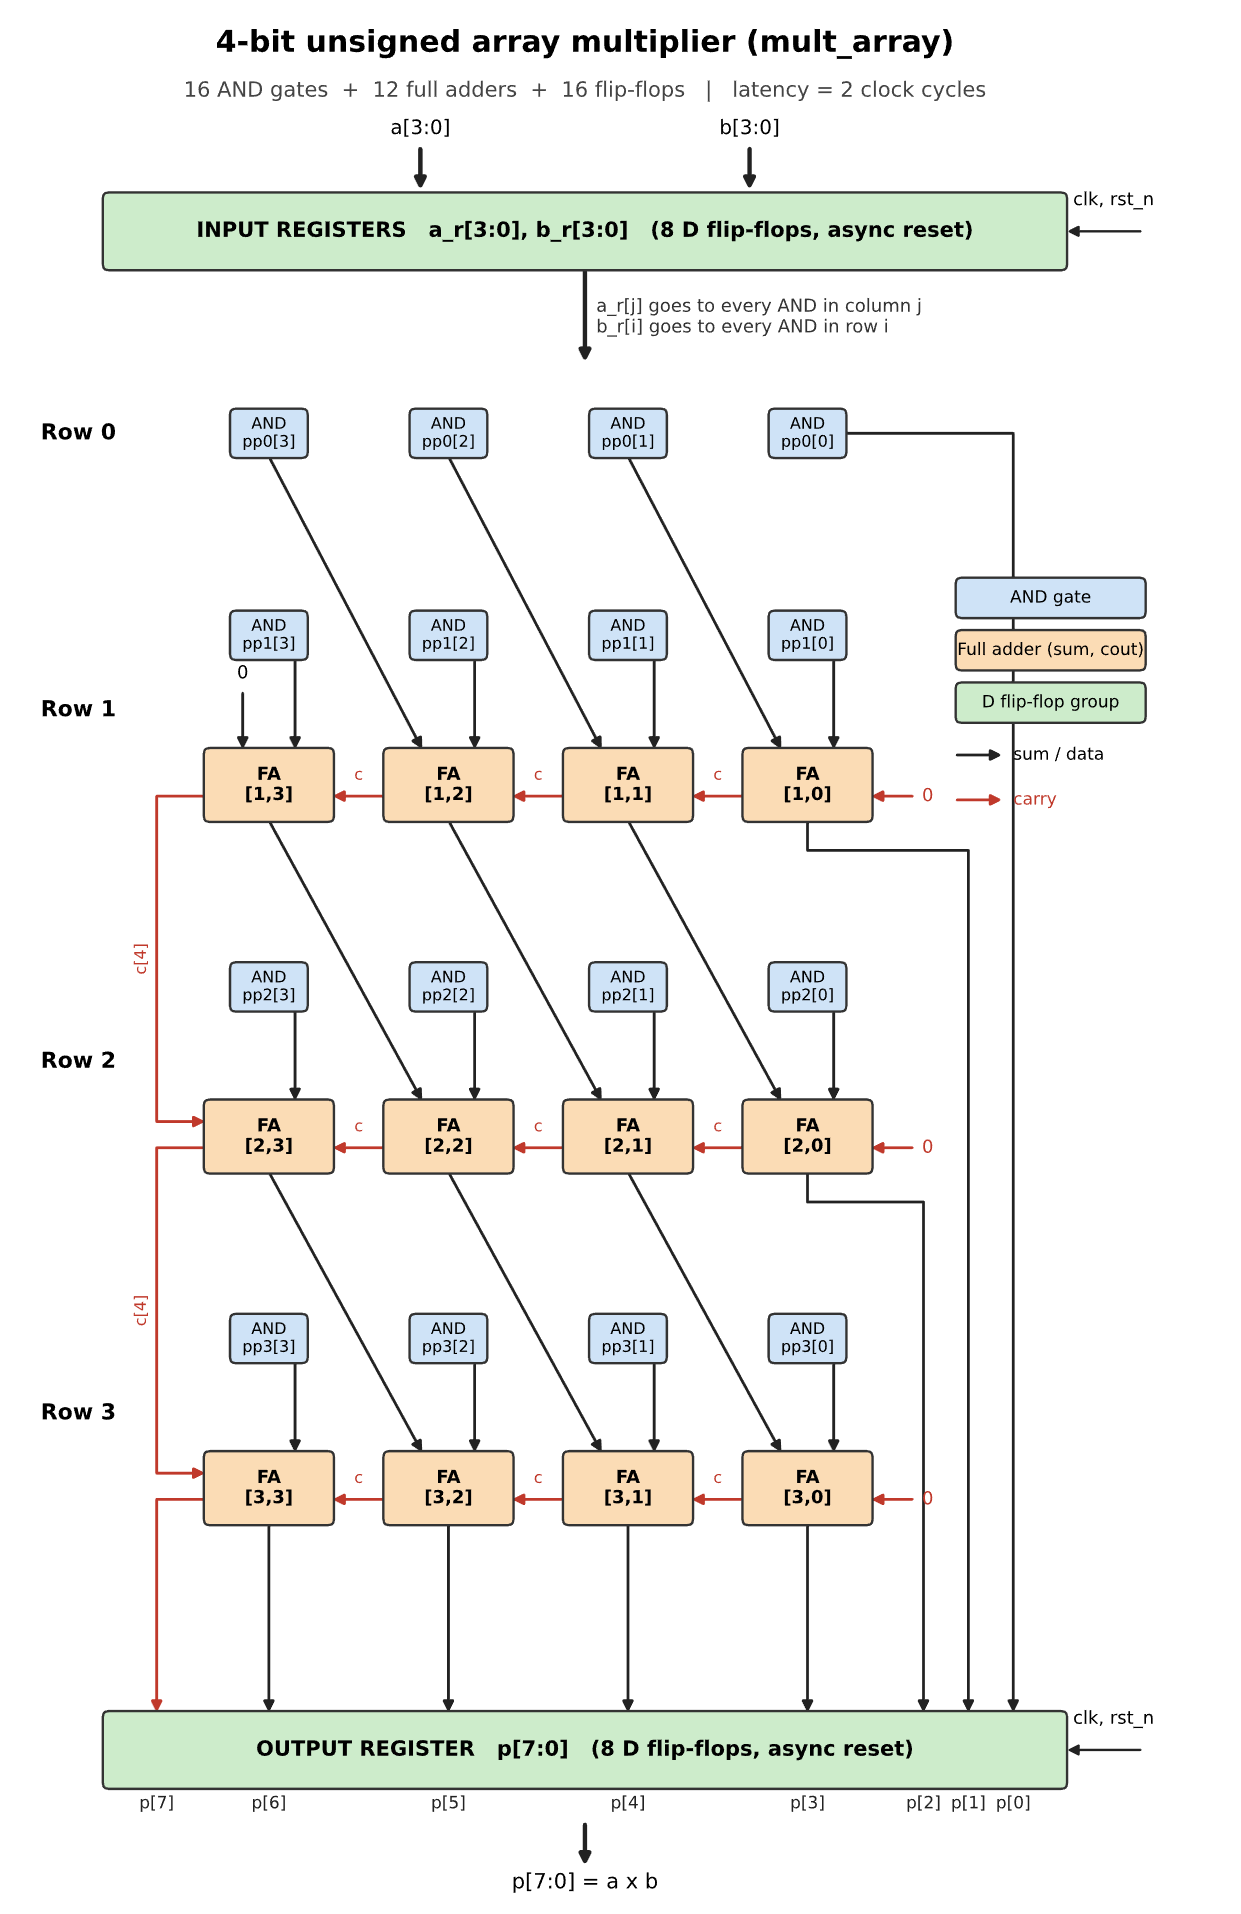
\includegraphics[width=0.92\columnwidth]{block_diagram.png}
\caption{Block diagram: 8 input flip-flops, 16 AND gates, 12 full adders in three ripple-carry rows (red arrows are carries), and 8 output flip-flops.}
\label{fig:block}
\end{figure}

\begin{figure*}[t]
\centering
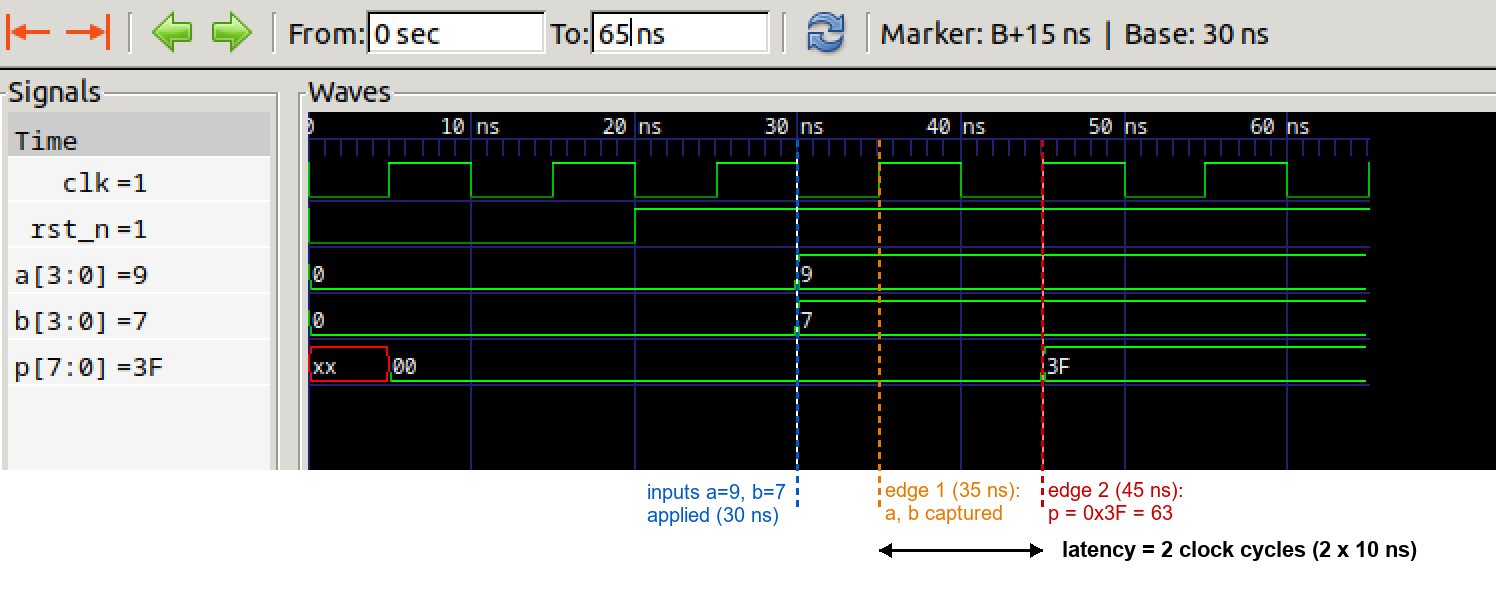
\includegraphics[width=0.86\textwidth]{waveform_latency.png}
\caption{GTKWave view of \texttt{clk}, \texttt{rst\_n}, \texttt{a}, \texttt{b} and \texttt{p} for A = 9, B = 7 (10\,ns clock period). The inputs change at 30\,ns and are captured at clock edge 1 (35\,ns). The product 0x3F = 63 appears on \texttt{p} at edge 2 (45\,ns), so the latency is 2 clock cycles (20\,ns).}
\label{fig:wave}
\end{figure*}

\subsection{Testbench}
\texttt{tb/tb\_mult.v} is \emph{exhaustive} (it tries every input) and \emph{self-checking} (it computes the expected answer and compares automatically). Table~\ref{tab:tb} lists each requirement and how the testbench meets it.

\begin{table}[!htbp]
\centering\footnotesize
\begin{tabularx}{\columnwidth}{>{\raggedright\arraybackslash}p{2.6cm}L}
\toprule
\textbf{Requirement} & \textbf{Implementation} \\
\midrule
10\,ns clock; reset for 2 cycles & \texttt{always \#5 clk = \textasciitilde clk}; \texttt{rst\_n} = 0 until the falling edge after the second rising edge (20\,ns). \\
All 256 input pairs & Nested loops \texttt{i, j} = 0\ldots15. \\
Respect the 2-cycle latency & Inputs change on a falling edge; the testbench waits two rising edges and checks \texttt{p} on the next falling edge, away from any clock edge. \\
Compare with \texttt{a * b} & \texttt{expected = i * j}; the \texttt{*} operator is used only here. \\
Report & One \texttt{MISMATCH} line per error, then exactly one \texttt{PASS:}/\texttt{FAIL:} summary line. \\
Waveform & \texttt{\$dumpfile("mult.vcd")}. \\
\bottomrule
\end{tabularx}
\caption{Testbench requirements and how \texttt{tb/tb\_mult.v} meets them.}
\label{tab:tb}
\end{table}
Each vector takes 3 clock cycles (30\,ns), so the run ends at $20\text{ ns} + 256 \times 30\text{ ns} = 7700$\,ns. This matches the simulator's \texttt{\$finish} time of 7\,700\,000\,ps.

\subsection{Simulation results and error test}
The RTL simulation prints \texttt{PASS: 256 vectors checked, 0 errors}, so the design is correct for every input.

A testbench is only useful if it can fail. To check this, \texttt{sum} in \texttt{full\_adder.v} was changed to \texttt{a \^{} b}, which ignores the carry-in. The testbench then printed \texttt{FAIL: 256 vectors checked, 95 errors}; Listing~\ref{lst:fail} in the Appendix shows the first mismatches. A vector can only fail when some full adder actually receives a carry-in of 1. Many vectors never create an internal carry (for example $a = 0$, $b = 0$, or an operand that is a power of two), which is why the other 161 vectors still pass. The change was then undone and the testbench prints PASS again.

\subsection{Hand-worked example}
A is the last digit of a roll number plus 5. Roll number 2023112014 ends in 4, so A = 9 = 1001$_2$, and B = 7 = 0111$_2$:
\begin{lstlisting}[basicstyle=\ttfamily\scriptsize]
            1 0 0 1     A = 9
          x 0 1 1 1     B = 7
    ---------------
            1 0 0 1     pp0 = A AND b0 (b0 = 1)
          1 0 0 1       pp1 = A AND b1 (b1 = 1), shifted 1
        1 0 0 1         pp2 = A AND b2 (b2 = 1), shifted 2
      0 0 0 0           pp3 = A AND b3 (b3 = 0), shifted 3
    ---------------
    0 0 1 1 1 1 1 1     P = 63
\end{lstlisting}
Table~\ref{tab:hand} computes the same product the way the hardware does, row by row, using the connections of Table~\ref{tab:conn}. Both methods give 0011\,1111$_2$ = 63 = 0x3F.

\begin{table}[!htbp]
\centering\footnotesize
\begin{tabular}{ccccl}
\toprule
\textbf{Row} & $pp_i$ & $+\,r_{i-1}$ & $=\{c, s\}$ & \textbf{Outputs} \\
\midrule
0 & \texttt{1001} & -- & -- & $p[0]=1$, $r_0=$ \texttt{0100} \\
1 & \texttt{1001} & \texttt{0100} & \texttt{0 1101} & $p[1]=1$, $r_1=$ \texttt{0110} \\
2 & \texttt{1001} & \texttt{0110} & \texttt{0 1111} & $p[2]=1$, $r_2=$ \texttt{0111} \\
3 & \texttt{0000} & \texttt{0111} & \texttt{0 0111} & $p[3]=1$, $p[7{:}4]=$ \texttt{0011} \\
\bottomrule
\end{tabular}
\caption{Row-by-row evaluation of $9 \times 7$ in the array (all values in binary). No full adder produces a carry for this input pair.}
\label{tab:hand}
\end{table}

\subsection{Waveform}
Fig.~\ref{fig:wave} shows this example in simulation:
\begin{enumerate}
  \item The inputs change to $a = 9$, $b = 7$ at 30\,ns.
  \item At clock edge 1 (35\,ns), the input registers capture them.
  \item During the next cycle, the array computes the product.
  \item At edge 2 (45\,ns), the output register captures 0x3F = 63.
\end{enumerate}
This shows the 2-cycle latency directly. Before 5\,ns, \texttt{p} shows \texttt{xx} (unknown). \texttt{rst\_n} starts at 0 without a falling edge, so the asynchronous-reset block first runs at the first clock edge, which then clears \texttt{p} to 00. This is a simulation start-up effect only.

% =====================================================================
\section{Synthesis (Part B)}

\subsection{What synthesis does}
\emph{Logic synthesis} turns the behavioural Verilog into a \emph{netlist}: a list of real cells from the SKY130 library and the wires between them. Each cell is a pre-designed gate whose area and delay are given in the \emph{Liberty} file (\texttt{.lib}). Table~\ref{tab:synth} lists the steps of \texttt{synth/synth.tcl}. The key step is \texttt{abc}: it does \emph{technology mapping}, choosing the combination of library gates that implements the logic with good area and delay. Because of \texttt{-flatten}, ABC sees the whole multiplier as one block of logic rather than 12 separate full adders, so it can optimise across adder boundaries.

\begin{table}[!htbp]
\centering\footnotesize
\begin{tabularx}{\columnwidth}{c>{\raggedright\arraybackslash}p{3.4cm}L}
\toprule
\textbf{Step} & \textbf{Yosys command} & \textbf{Purpose} \\
\midrule
1 & \texttt{read\_verilog} & Read the two RTL files \\
2 & \texttt{synth -top mult\_array -flatten} & Generic synthesis; merge the full adders into one module \\
3 & \texttt{dfflibmap -liberty \$lib} & Map the 16 flip-flops to SKY130 cells \\
4 & \texttt{abc -liberty \$lib} & Map the logic to SKY130 gates \\
5 & \texttt{opt\_clean -purge} & Remove unused wires \\
6 & \texttt{tee -o \ldots{} stat -liberty \$lib} & Write the cell and area report \\
7 & \texttt{write\_verilog -noattr} & Write the gate-level netlist \\
\bottomrule
\end{tabularx}
\caption{Steps of \texttt{synth/synth.tcl}, run with \texttt{yosys -c synth/synth.tcl}.}
\label{tab:synth}
\end{table}

\subsection{Results}
Table~\ref{tab:partB} gives the required results. The flip-flops are \texttt{dfrtp\_1} cells: D flip-flops with an active-low asynchronous reset (the \texttt{\_1} suffix is the drive strength). The 47 logic cells are:
\begin{itemize}
  \item 10 XOR/XNOR cells and 3 \texttt{maj3} cells. These are the full adders' sum and carry functions.
  \item 6 AND cells.
  \item 16 NAND/NOR cells.
  \item 10 complex gates, such as \texttt{a21oi} $= \overline{A_1A_2 + B_1}$ and \texttt{o311ai} $= \overline{(A_1+A_2+A_3)B_1C_1}$. In these names, ``a'' is AND, ``o'' is OR and ``i'' means an inverted output.
  \item 2 inverters.
\end{itemize}
Table~\ref{tab:cells} in the Appendix lists every cell with its area.

\begin{table}[!htbp]
\centering\footnotesize
\begin{tabularx}{\columnwidth}{>{\raggedright\arraybackslash}p{3.3cm}L}
\toprule
\textbf{Metric} & \textbf{Value} \\
\midrule
Total number of cells & 63 cells \\
Number of flip-flops & 16 cells (\texttt{dfrtp\_1}) \\
Total cell area & 740.71\umsq \\
Flip-flop area & 400.38\umsq{} ($16 \times 25.024$\umsq) \\
Flip-flop area (\% of total) & 54.05\,\% \\
3 most-used cell types & \texttt{dfrtp\_1} $\times$ 16, \texttt{nand2\_1} $\times$ 8, \texttt{a21oi\_1} $\times$ 6 \\
Netlist simulation result & \texttt{PASS: 256 vectors checked, 0 errors} \\
\bottomrule
\end{tabularx}
\caption{Part B results (from \texttt{synth/mult\_array\_stat.rpt}).}
\label{tab:partB}
\end{table}

\subsection{Gate-level simulation}
Synthesis could in principle change the behaviour, for example if a register were mis-mapped. To rule this out, the synthesised netlist was simulated with the \emph{same} testbench, using the SKY130 Verilog cell models (\texttt{primitives.v}, \texttt{sky130\_fd\_sc\_hd.v}). \texttt{-DFUNCTIONAL} selects the logic-only cell models, and \texttt{-DUNIT\_DELAY=\#1} gives every cell a small unit delay (\texttt{\#1}) so that signals change in a clean order. The result is again \texttt{PASS: 256 vectors checked, 0 errors} (Listing~\ref{lst:gls}), so the netlist behaves exactly like the RTL.

% =====================================================================
\section{Timing (Part C)}

\subsection{Static timing analysis}
\emph{Static timing analysis} (STA) checks speed without simulation. It looks at every path from one flip-flop to the next and adds up the cell delays from the Liberty file.

A path launched at one clock edge must reach the next flip-flop before the following edge, so the \emph{setup} condition is
\begin{equation*}
t_{clk\to Q} + t_{logic} + t_{setup} \le T.
\end{equation*}
Here $t_{clk\to Q}$ is the time the launching flip-flop takes to update its output, $t_{logic}$ is the delay through the gates, and $t_{setup}$ is how long the data must be stable before the capturing edge.

The \emph{slack} is the required time ($T - t_{setup}$) minus the arrival time. Positive slack means the path meets timing; negative slack means it fails. The \emph{worst negative slack} (WNS) is the smallest slack in the design, and the path that has it is the \emph{critical path}.

\texttt{sta/sta.tcl} performs these steps:
\begin{enumerate}
  \item Read the typical-corner library and the Part B netlist.
  \item Create a clock of period $T$ on \texttt{clk}.
  \item Set an input delay and an output delay of 1.0\,ns. These model logic outside the chip, so the I/O paths are also checked.
  \item Report the worst slack and the critical path.
\end{enumerate}
The clock is \emph{ideal}: it arrives at every flip-flop at the same time. There are no wire delays, because the design has not been placed yet.

\subsection{Maximum frequency}
At $T = 10$\,ns the worst slack is +7.396\,ns, so the circuit could run 7.396\,ns faster:
\begin{gather*}
T_{\min} = 10\text{ ns} - 7.396\text{ ns} = 2.604\text{ ns},\\
F_{\max} = 1000 / 2.604 = 384.02\text{ MHz}.
\end{gather*}
Re-running at $T = 2.60$\,ns (T$_{\min}$ rounded to 0.01\,ns) gives a slack of $-0.004$\,ns. That is effectively zero, which confirms \Tmin; the 0.004\,ns comes only from rounding 2.604\,ns down to 2.60\,ns. Table~\ref{tab:partC} summarises the results.

\begin{table}[!htbp]
\centering\footnotesize
\begin{tabularx}{\columnwidth}{>{\raggedright\arraybackslash}p{3.3cm}L}
\toprule
\textbf{Metric} & \textbf{Value} \\
\midrule
Worst slack at $T = 10$\,ns & +7.396\,ns \\
\Tmin & 2.604\,ns \\
\Fmax & 384.02\,MHz \\
Slack at $T = 2.60$\,ns & $-0.004$\,ns ($\approx 0$\,ns) \\
Critical path start point & \texttt{\_095\_} = input register \texttt{a\_r[1]} \\
Critical path end point & \texttt{\_092\_} = output register \texttt{p[6]} \\
Cells on the critical path & 10 cells (2 flip-flops + 8 gates) \\
Latency $= 2 \times T_{\min}$ & 5.208\,ns \\
Throughput & 384.02 million results per second \\
\bottomrule
\end{tabularx}
\caption{Part C results (OpenSTA, typical corner, pre-layout).}
\label{tab:partC}
\end{table}

\subsection{Critical path}
Table~\ref{tab:path} lists the critical path cell by cell. The instance names (\texttt{\_095\_}, \texttt{\_092\_}) are generated by Yosys. Tracing them in the netlist shows that they are the flip-flops for \texttt{a\_r[1]} and \texttt{p[6]}.

\begin{table}[!htbp]
\centering\footnotesize
\begin{tabular}{cllp{1.75cm}rr}
\toprule
\textbf{\#} & \textbf{Cell} & \textbf{Signal} & \textbf{Part of} & \textbf{Incr (ns)} & \textbf{Arr. (ns)} \\
\midrule
1 & \texttt{dfrtp\_1} & \texttt{a\_r[1]} & launch FF & 0.398 & 0.398 \\
2 & \texttt{clkinv\_1} & $\overline{a\_r[1]}$ & AND gates & 0.074 & 0.472 \\
3 & \texttt{o311ai\_0} & merged & ANDs + fa1\_1 & 0.348 & 0.820 \\
4 & \texttt{a21oi\_1} & $c_2[1]$ & fa2\_0 carry & 0.172 & 0.992 \\
5 & \texttt{maj3\_1} & $c_2[2]$ & fa2\_1 carry & 0.381 & 1.373 \\
6 & \texttt{xnor2\_1} & $\overline{s_2[2]}$ & fa2\_2 sum & 0.160 & 1.534 \\
7 & \texttt{maj3\_1} & $\overline{c_3[2]}$ & fa3\_1 carry & 0.385 & 1.918 \\
8 & \texttt{maj3\_1} & $\overline{c_3[3]}$ & fa3\_2 carry & 0.377 & 2.295 \\
9 & \texttt{xnor3\_1} & $s_3[3]$ & fa3\_3 sum & 0.175 & 2.471 \\
10 & \texttt{dfrtp\_1} & \texttt{p[6]} & capture FF & 0.000 & 2.471 \\
\bottomrule
\end{tabular}
\caption{Critical path at $T = 2.60$\,ns (\texttt{sta/mult\_array\_timing.rpt}). fa$r$\_$c$ is the full adder in row $r$, column $c$; an overline marks a signal ABC built inverted. The capture flip-flop needs 0.134\,ns of setup, so the required time is $2.600 - 0.134 = 2.466$\,ns and the slack is $2.466 - 2.471 = -0.004$\,ns.}
\label{tab:path}
\end{table}

\textbf{Identifying each gate.} Because Yosys flattened the full adders, the netlist gates carry generated names, not adder names. To find what each gate computes, the netlist was evaluated for all 256 values of (\texttt{a\_r}, \texttt{b\_r}). The truth table of every net on the path was then compared with every partial product, sum and carry of the RTL (Section~2.1). The result is the ``Signal'' column of Table~\ref{tab:path}.

\textbf{Reading the path.} Bit $a[1]$ leaves its register and enters the partial products. The \texttt{o311ai} merges partial-product ANDs with full adder fa1\_1. Its sum $s_1[1]$ is passed down as $r_1[0]$ into fa2\_0. The signal then ripples along the row-2 carry chain (fa2\_0 $\to$ fa2\_1 $\to$ fa2\_2). The sum $s_2[2]$ of fa2\_2 is passed down as $r_2[1]$ into fa3\_1. Finally, the signal ripples along the row-3 carry chain (fa3\_1 $\to$ fa3\_2 $\to$ fa3\_3) to the top sum bit $s_3[3] = p[6]$. ABC built some carries and sums inverted, because inverting CMOS gates are smaller and faster; the next gate absorbs the inversion.

\textbf{Comparison with $2N$.} The path crosses \textbf{7 full-adder stages}: fa1\_1, fa2\_0, fa2\_1, fa2\_2, fa3\_1, fa3\_2 and fa3\_3. Six of the eight gates compute a full-adder carry or sum directly, and the \texttt{o311ai} contains fa1\_1. Seven stages agree well with the estimate of about $2N = 8$ full-adder delays, which is only an approximation of the longest chain. The 8 gates contribute 2.073\,ns of logic delay ($2.471 - 0.398$), or about 0.30\,ns per stage. Each stage costs a single gate because the path needs either the carry or the sum of each adder, never both: a carry is one \texttt{maj3} (or AOI) cell and a sum is one \texttt{xnor} cell.

\textbf{Other paths.} The input-to-register paths (1.0\,ns input delay straight into a flip-flop) and register-to-output paths (CLK$\to$Q plus 1.0\,ns output delay) are short. The asynchronous-reset \emph{recovery} check, which requires the reset to be released a minimum time before the clock edge, has +9.228\,ns of slack at 10\,ns and +1.828\,ns at 2.60\,ns. Neither limits the clock.

% =====================================================================
\section{Physical Design (Part D)}

\begin{figure*}[t]
\centering
\begin{minipage}[b]{0.40\textwidth}\centering
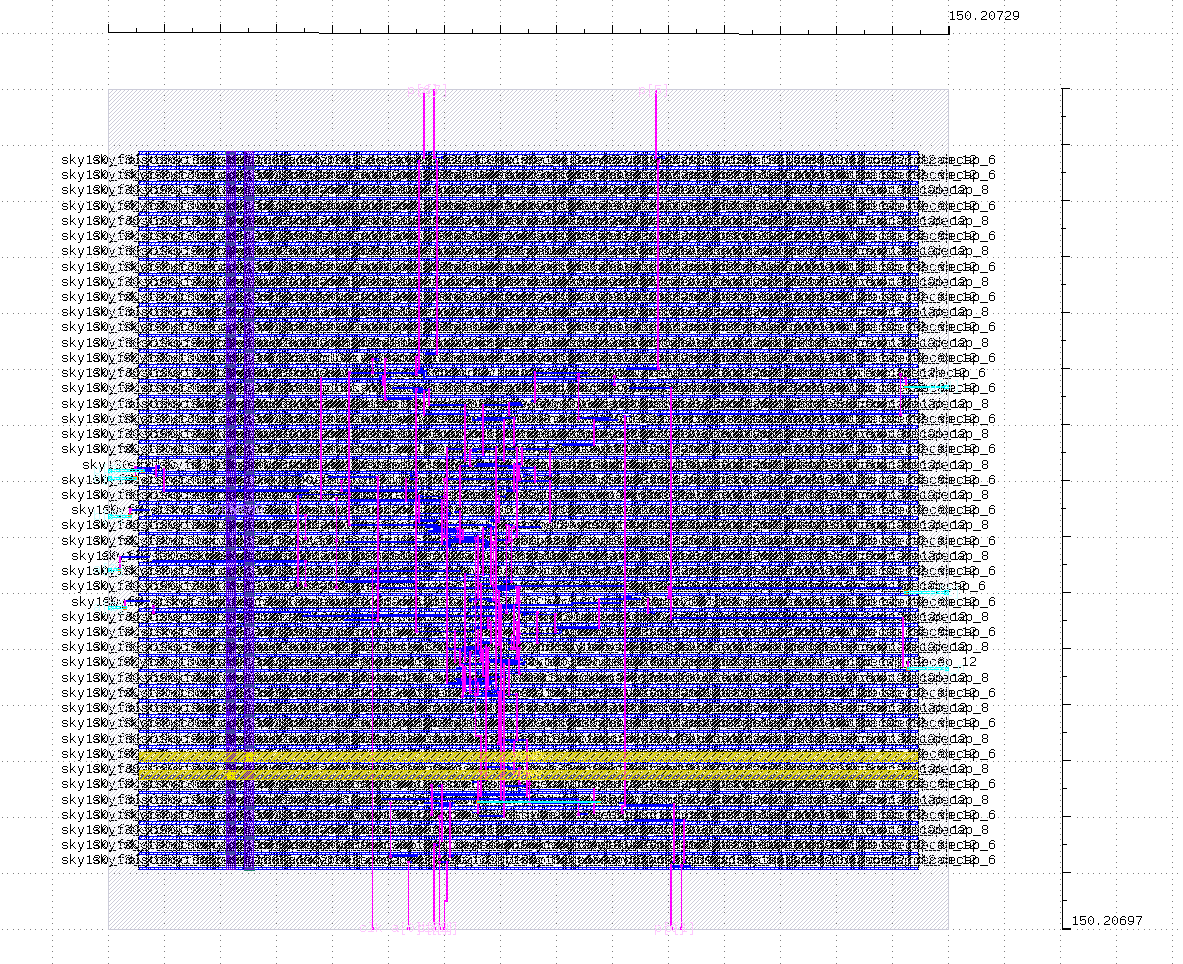
\includegraphics[width=\textwidth]{klayout_full_die.png}\\[-2pt]
{\footnotesize (a) whole die}
\end{minipage}\hfill
\begin{minipage}[b]{0.57\textwidth}\centering
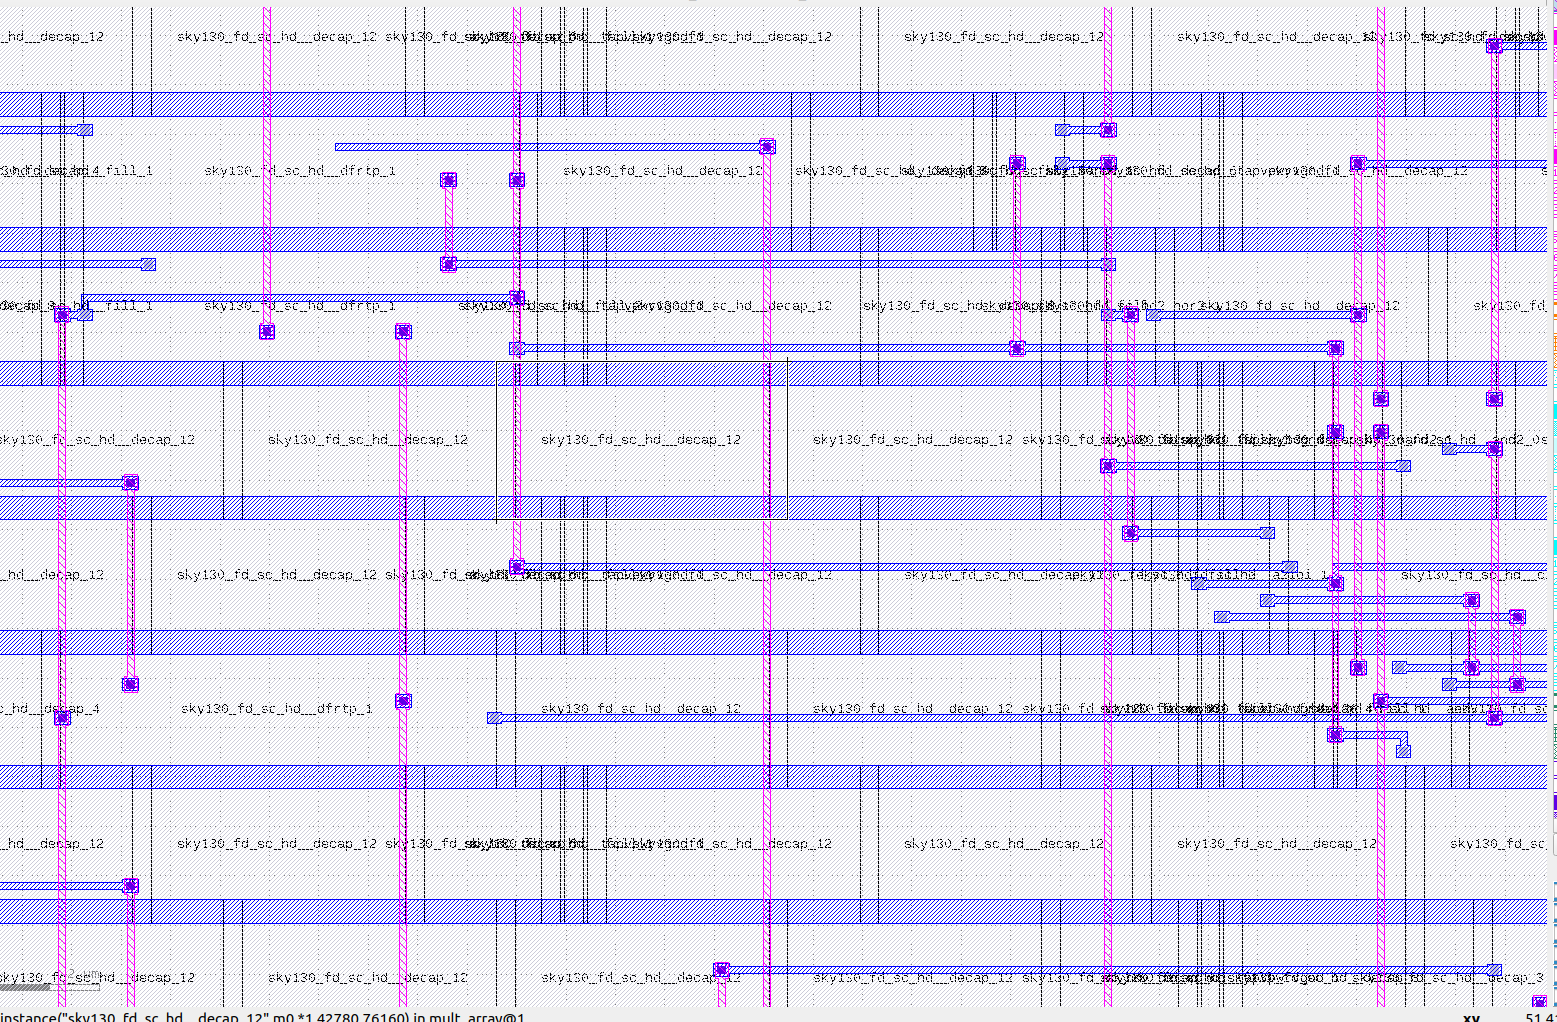
\includegraphics[width=\textwidth]{klyaout_zoom.png}\\[-2pt]
{\footnotesize (b) zoomed view}
\end{minipage}
\caption{Final layout in KLayout. (a) The 150\,$\mu$m $\times$ 150\,$\mu$m die: 47 standard-cell rows filled with tap, decap and filler cells, with the routed logic in the centre and wires running to the I/O pins on the edges. (b) Zoomed view: the VPWR/VGND rails bound each row, which holds standard cells (e.g.\ \texttt{dfrtp\_1}, \texttt{decap\_12}). Metal wires and vias connect the cell pins.}
\label{fig:layout}
\end{figure*}

\subsection{The flow}
LibreLane turns the RTL into a manufacturable layout in about 80 automatic steps. It was run with \texttt{-{}-pdk sky130A -{}-scl sky130\_fd\_sc\_hd}, because the container's default PDK is a different one. Table~\ref{tab:flow} explains the main stages.

\begin{table}[!htbp]
\centering\footnotesize
\begin{tabularx}{\columnwidth}{>{\raggedright\arraybackslash}p{2.0cm}L}
\toprule
\textbf{Stage} & \textbf{What it does} \\
\midrule
Synthesis & RTL to standard cells, as in Part B \\
Floorplan & Fixes the die (whole chip) at 150\,$\mu$m $\times$ 150\,$\mu$m and the core (where cells go) at 17\,759.5\umsq; creates 47 placement rows \\
Power grid & Lays out the VPWR (1.8\,V) and VGND (0\,V) supply rails \\
Tap/decap & Inserts well-tap and decoupling cells \\
Placement & Puts every cell at a legal site in the rows \\
CTS & Clock-tree synthesis: buffers the clock so it reaches all 16 flip-flops at nearly the same time; the difference in arrival is the \emph{skew} \\
Timing repair & Resizes gates and inserts buffers to fix setup, slew and load violations \\
Routing & Draws the metal wires and vias between pins \\
Extraction & Computes each wire's resistance and capacitance (parasitics) \\
Signoff & STA with real wires at 9 corners; DRC (Magic, KLayout); LVS (Netgen); antenna and IR-drop checks \\
GDSII & Writes the final layout file sent to the foundry \\
\bottomrule
\end{tabularx}
\caption{Main stages of the LibreLane Classic flow.}
\label{tab:flow}
\end{table}

\texttt{pnr/config.json} contains exactly the required keys:
\begin{itemize}
  \item \texttt{DESIGN\_NAME = "mult\_array"}
  \item the two RTL files
  \item \texttt{CLOCK\_PORT = "clk"}
  \item \texttt{CLOCK\_PERIOD}
  \item \texttt{FP\_SIZING = "absolute"}
  \item \texttt{DIE\_AREA = [0, 0, 150, 150]}
\end{itemize}

\textbf{Corners.} Manufacturing and operating conditions vary, so signoff STA is run at 9 \emph{corners}:
\begin{itemize}
  \item three process/voltage/temperature (PVT) conditions: typical (tt, 1.80\,V, 25\,$^\circ$C), slow (ss, 1.60\,V, 100\,$^\circ$C) and fast (ff, 1.95\,V, $-40$\,$^\circ$C);
  \item each combined with minimum, nominal and maximum wire RC.
\end{itemize}
The chip must meet timing at all of them. Setup is hardest at the slow corner, and hold at the fast corner.

\subsection{Timing closure}
The first period is $1.2 \times T_{\min} = 1.2 \times 2.604\text{ ns} = 3.125$\,ns, rounded up to the next 0.5\,ns, which is 3.5\,ns. The 20\,\% margin over \Tmin{} allows for wires and the clock tree. After each run that failed setup, the period was increased by 0.5\,ns. Table~\ref{tab:runs} lists all 10 runs; 8.0\,ns is the first period that passes.

\begin{table}[!htbp]
\centering\footnotesize
\begin{tabular}{crrrrl}
\toprule
\textbf{Run} & \textbf{Period} & \textbf{Setup} & \textbf{Hold} & \textbf{Wire-} & \textbf{Result} \\
 & \textbf{(ns)} & \textbf{slack (ns)} & \textbf{slack (ns)} & \textbf{length ($\mu$m)} & \\
\midrule
1 & 3.5 & $-2.184$ & +0.114 & 2674 & FAIL \\
2 & 4.0 & $-1.684$ & +0.133 & 2674 & FAIL \\
3 & 4.5 & $-1.184$ & +0.135 & 2675 & FAIL \\
4 & 5.0 & $-0.682$ & +0.135 & 2675 & FAIL \\
5 & 5.5 & $-0.208$ & +0.135 & 2688 & FAIL \\
6 & 6.0 & $-0.154$ & +0.135 & 2612 & FAIL \\
7 & 6.5 & $-0.224$ & +0.136 & 2568 & FAIL \\
8 & 7.0 & $-0.137$ & +0.136 & 2560 & FAIL \\
9 & 7.5 & $-0.100$ & +0.136 & 2499 & FAIL \\
\textbf{10} & \textbf{8.0} & \textbf{+0.400} & +0.136 & 2499 & \textbf{PASS} \\
\bottomrule
\end{tabular}
\caption{All LibreLane runs. Slack is the worst over the 9 signoff corners. Every run has 0 DRC errors and 0 LVS errors; FAIL means setup slack $<$ 0\,ns.}
\label{tab:runs}
\end{table}

\textbf{Why the slack changes unevenly.} The timing-repair step runs after clock-tree synthesis but \emph{before} routing, and only aims for a 0.05\,ns setup margin. Routing then adds real wire delay, which takes some slack back at the slow corner. This explains three regimes in Table~\ref{tab:runs}:
\begin{itemize}
  \item \textbf{3.5 to 5.0\,ns:} repair cannot close timing (at 3.5\,ns it reaches only $-2.02$\,ns before routing). Nothing else changes between runs, so each 0.5\,ns increase in the period improves the final slack by exactly 0.5\,ns.
  \item \textbf{5.5 to 7.5\,ns:} repair can close timing, but only just. At 6.0\,ns it reaches +0.068\,ns before routing; routing then costs 0.22\,ns, leaving $-0.154$\,ns (Listing~\ref{lst:rsz}). All runs in this range end in a narrow band between $-0.10$\,ns and $-0.22$\,ns.
  \item \textbf{8.0\,ns:} the design meets timing before routing without any repair, so real margin is left (+0.400\,ns).
\end{itemize}
The synthesised logic is identical in every run (16 flip-flops, 42 multi-input cells, 4 inverters). Only the number of buffers changes, from 33 at 3.5\,ns to 21 at 8.0\,ns (including the 17 I/O port buffers, which are present in every run). Because the failing runs are so close to 0\,ns, small differences in tool version, netlist or placement can move the passing period by 0.5 to 1.5\,ns.

\begin{table}[!htbp]
\centering\footnotesize
\begin{tabularx}{\columnwidth}{>{\raggedright\arraybackslash}p{2.9cm}L}
\toprule
\textbf{Metric} & \textbf{Value} \\
\midrule
CLOCK\_PERIOD used & 8.0\,ns \\
Number of runs needed & 10 runs \\
Core area & 17\,759.5\umsq{} (die 22\,500\umsq) \\
Cells after synthesis (Part B) & 63 cells \\
Cells after place and route & 1883 instances: 86 logic, flip-flop and buffer cells, 245 tap cells, 1552 decap and filler cells \\
Kinds of cells added & \texttt{buf\_2} (17 I/O port buffers), \texttt{clkdlybuf4s*} (4 repair buffers), \texttt{clkbuf\_16} (3 clock buffers), \texttt{tapvpwrvgnd\_1} (245), \texttt{decap\_*} (1298), \texttt{fill\_*} (254) \\
Wirelength & 2499\um{} (561 vias) \\
Setup slack & +0.400\,ns (corner \texttt{max\_ss\_100C\_1v60}) \\
Post-route \Fmax & $1000/(8.0 - 0.400) = 131.58$\,MHz \\
\Fmax{} from Part C & 384.02\,MHz \\
DRC errors & 0 errors (Magic and KLayout) \\
LVS errors & 0 errors (Netgen) \\
\bottomrule
\end{tabularx}
\caption{Part D results for the final run (from \texttt{pnr/metrics.json}).}
\label{tab:partD}
\end{table}

\subsection{Cells added by place and route}
Synthesis produced 63 cells, but the final layout has 1883 instances. LibreLane re-synthesises the RTL with its own script, which gives 62 cells. It then adds 17 I/O port buffers, 4 repair buffers and 3 clock buffers, so the layout has $62 + 17 + 4 + 3 = 86$ functional cells. Everything else is support cells, as Table~\ref{tab:added} shows. The cells occupy only 1264.96\umsq{} of the 17\,759.5\umsq{} core (7.1\,\% utilisation), so most of the core is filled with filler and decap cells.

\begin{table}[!htbp]
\centering\footnotesize
\begin{tabularx}{\columnwidth}{>{\raggedright\arraybackslash}p{1.45cm}rrL}
\toprule
\textbf{Class} & \textbf{Count} & \textbf{Area ($\mu$m$^2$)} & \textbf{Why it is needed} \\
\midrule
I/O port buffers & 17 & 85.1 & One \texttt{buf\_2} on each of the 9 inputs (\texttt{rst\_n}, \texttt{a}, \texttt{b}) and 8 outputs (\texttt{p}); isolates the internal logic from unknown external loads and drivers \\
Repair buffers & 4 & 40.0 & \texttt{clkdlybuf4s*}; split heavily loaded nets (most likely \texttt{rst\_n}, which drives all 16 flip-flops) to fix slew and load limits \\
Clock buffers & 3 & 75.1 & Drive 16 clock pins with sharp edges and low skew \\
Tap cells & 245 & 306.5 & Tie the n-well to VPWR and the substrate to VGND, preventing latch-up \\
Decap cells & 1298 & \multirow{2}{*}{16\,494.6} & Charge reservoirs between VPWR and VGND that reduce supply noise \\
Filler cells & 254 & & Keep wells, implants and power rails continuous across gaps (needed for DRC) \\
\bottomrule
\end{tabularx}
\caption{Cells added by the flow, with their total area and purpose.}
\label{tab:added}
\end{table}

\subsection{Signoff}
Table~\ref{tab:partD} gives the required results, and Table~\ref{tab:corners} shows the slack at each corner.
\begin{itemize}
  \item Setup is limited by the slow corner (+0.400\,ns), and hold by the fast corner (+0.136\,ns).
  \item The typical corner has 4.2\,ns of setup slack to spare.
  \item Clock skew is about 0.26\,ns.
  \item There are 0 antenna violations and 0 power-grid violations.
  \item The worst IR drop (voltage lost along the power rails) is 0.31\,mV.
  \item Total power at the typical corner is 0.296\,mW.
  \item The flow reports 11 max-slew warnings at the slow corners. These are not setup or hold violations.
\end{itemize}
Fig.~\ref{fig:layout} shows the final layout.

\begin{table}[!htbp]
\centering\footnotesize
\begin{tabular}{llrrr}
\toprule
\textbf{Corner} & \textbf{RC} & \textbf{Setup (ns)} & \textbf{Hold (ns)} & \textbf{\Fmax{} (MHz)} \\
\midrule
\multirow{3}{*}{tt, 1.80\,V, 25\,$^\circ$C} & min & 4.267 & 0.360 & 267.9 \\
 & nom & 4.240 & 0.370 & 265.9 \\
 & max & 4.209 & 0.377 & 263.8 \\
\midrule
\multirow{3}{*}{ss, 1.60\,V, 100\,$^\circ$C} & min & 0.500 & 0.945 & 133.3 \\
 & nom & 0.449 & 0.963 & 132.4 \\
 & max & \textbf{0.400} & 0.974 & \textbf{131.6} \\
\midrule
\multirow{3}{*}{ff, 1.95\,V, $-40$\,$^\circ$C} & min & 5.535 & \textbf{0.136} & 405.8 \\
 & nom & 5.526 & 0.143 & 404.2 \\
 & max & 5.519 & 0.147 & 403.1 \\
\bottomrule
\end{tabular}
\caption{Setup and hold slack at the 9 signoff corners of the final run (period 8.0\,ns). $F_{\max} = 1000/(8.0 - \text{setup slack})$.}
\label{tab:corners}
\end{table}

% =====================================================================
\section{Answers to Questions}

\q{Q1. The array needs 16 AND gates and 12 full adders. How many cells did synthesis produce for the logic, and why is it not 16 + 12?}
Synthesis produced $63 - 16 = 47$ logic cells (340.3\umsq), not 28. ``AND gate'' and ``full adder'' are RTL building blocks, not single library cells. With \texttt{-flatten}, the module boundaries disappear and ABC re-implements the whole Boolean function with whatever cells give a good area and delay. Four effects explain the count:
\begin{itemize}
  \item \textbf{A full adder needs at least two cells:} a sum cell (\texttt{xor2}, \texttt{xnor2}, \texttt{xor3} or \texttt{xnor3}; 10 in total) and a carry cell (\texttt{maj3}) or an equivalent NAND/AOI network. That alone is about 24 cells for 12 full adders.
  \item \textbf{AND gates are absorbed} into compound gates such as \texttt{a21oi}, \texttt{a22oi}, \texttt{o311ai}, \texttt{nand3} and \texttt{nand4}. Only 6 plain AND cells remain.
  \item \textbf{Constant inputs simplify some adders.} The carry into every row ($c_i[0] = 0$) and the top bit of $r_0$ are 0, so those full adders become half adders (an \texttt{xor2} plus a \texttt{nand2} or \texttt{and2}).
  \item \textbf{Inverting cells need a few inverters} (\texttt{clkinv}, \texttt{nand2b}, \texttt{nor2b}).
\end{itemize}

\q{Q2. What is the critical path, how many cells are on it, and how does it compare with about 2N full-adder delays?}
It runs from input register \texttt{a\_r[1]} (\texttt{\_095\_}) to output register \texttt{p[6]} (\texttt{\_092\_}). It has 10 cells: the launching flip-flop, 8 gates (\texttt{clkinv}, \texttt{o311ai}, \texttt{a21oi}, \texttt{maj3}, \texttt{xnor2}, \texttt{maj3}, \texttt{maj3}, \texttt{xnor3}) and the capturing flip-flop. The data arrives after 2.471\,ns, giving $T_{\min} = 2.604$\,ns. Matching every net to the RTL by truth table (Table~\ref{tab:path}) shows that the path crosses \textbf{7 full-adder stages}: along the row-2 carry chain, down through $s_2[2]$, and along the row-3 carry chain to $s_3[3] = p[6]$. Six of the 8 gates compute a full-adder carry or sum directly. Seven stages are close to the estimate of $2N = 8$ full-adder delays. Each stage costs only one gate (about 0.30\,ns), because the path uses either the carry or the sum of each adder, not both.

\q{Q3. What percentage of the cell area is flip-flops, and why is it so large?}
Flip-flops take 400.38\umsq{} of 740.71\umsq{}, which is 54.05\,\%, although they are only 16 of the 63 cells (25\,\%). There are two reasons:
\begin{itemize}
  \item \textbf{A flip-flop is a large cell.} One \texttt{dfrtp\_1} is 25.02\umsq: 6.7 times a \texttt{nand2\_1} (3.75\umsq) and 3.5 times the average logic cell (7.24\umsq). An edge-triggered flip-flop with asynchronous reset is two latches plus clock buffering and reset logic, a few dozen transistors against 4 for a NAND2.
  \item \textbf{Scaling.} The array logic grows as $N^2$ (16 ANDs and 12 adders), while the registers grow only as $4N$ (16 flip-flops). At $N = 4$ the logic is still small, so the registers dominate. At 8 bits the share falls to about 35\,\% (Q6).
\end{itemize}

\q{Q4. Why is the post-route \Fmax{} lower than in Part C? Which cells did the flow add, and why?}
The post-route \Fmax{} is 131.58\,MHz, against 384.02\,MHz from Part C, about 2.9 times lower. The two numbers are measured under very different conditions:
\begin{enumerate}
  \item \textbf{Corner.} Part C used only the typical library. Signoff reports the worst of 9 corners, which is slow-slow at 1.60\,V and 100\,$^\circ$C, where transistors are about half as fast. In the same run, the typical corner alone allows $1000/(8.0 - 4.240) \approx 266$\,MHz.
  \item \textbf{Wires.} Part C had no parasitics. After routing, 2499\um{} of wire and 561 vias add resistance and capacitance to every net, and the pins sit on the edge of a 150\um{} die.
  \item \textbf{Clock tree.} Part C assumed an ideal clock. The real tree has insertion delay and about 0.26\,ns of skew.
  \item \textbf{Constraints.} LibreLane's constraints are stricter: input and output delays are 20\,\% of the period (1.6\,ns at 8.0\,ns, against 1.0\,ns in Part C), plus 0.25\,ns of clock uncertainty and a 5\,\% timing derate.
  \item \textbf{Netlist.} LibreLane re-synthesises the design (62 cells instead of 63) and inserts buffers, so the post-route critical path is not the same as in Part C.
\end{enumerate}
The added cells and their purposes are listed in Table~\ref{tab:added}: I/O port buffers, repair buffers, clock buffers, tap cells, decap cells and filler cells.

\q{Q5. What do DRC and LVS verify, and why must both pass?}
\textbf{DRC} (design rule check) verifies the \emph{geometry} of the layout against the foundry's rules for every layer: minimum widths, spacings, enclosures, overlaps, density and antenna ratios. These rules describe what the factory can print reliably, and a violation can cause shorts, opens or very low yield.

\textbf{LVS} (layout versus schematic) extracts the transistors and their connections from the layout and checks that they form exactly the circuit in the netlist: same devices, same nets, same pins.

The two checks cover different risks. A layout can be manufacturable but the wrong circuit, or the right circuit but impossible to manufacture. A mask set is expensive and cannot be fixed after tape-out, so both must pass first. Our layout has 0 DRC errors in Magic and KLayout (the router's 6 first-pass violations were fixed in its second pass), 0 LVS errors in Netgen, and 0 antenna violations.

\q{Q6. Estimate how the full adders and critical path change at 8 bits.}
Table~\ref{tab:scale} applies the formulas from the assignment to $N = 8$.

\begin{table}[!htbp]
\centering\footnotesize
\begin{tabular}{llrrr}
\toprule
\textbf{Quantity} & \textbf{Formula} & \textbf{$N = 4$} & \textbf{$N = 8$} & \textbf{Change} \\
\midrule
AND gates & $N^2$ & 16 & 64 & $\times 4$ \\
Full adders & $N(N-1)$ & 12 & 56 & $\times 4.67$ \\
Flip-flops & $4N$ & 16 & 32 & $\times 2$ \\
Critical path & $2N$ FA delays & 8 & 16 & $\times 2$ \\
\bottomrule
\end{tabular}
\caption{Scaling from 4 to 8 bits (counts in cells; path length in full-adder delays).}
\label{tab:scale}
\end{table}

From Part C, the critical path crosses 7 full-adder stages in 2.073\,ns of logic, so one stage costs $2.073\text{ ns} / 7 = 0.296$\,ns. The flip-flop overhead is $0.398\text{ ns} + 0.134\text{ ns} = 0.532$\,ns (CLK$\to$Q plus setup). Using the $2N = 16$ estimate for $N = 8$:
\begin{gather*}
T_{\min} \approx 0.532 + 16 \times 0.296 = 5.27\text{ ns},\\
F_{\max} \approx 1000 / 5.27 = 190\text{ MHz}.
\end{gather*}
The number of full adders grows quadratically, by 4.7 times, but the critical path grows only linearly, by about 2 times, so \Tmin{} roughly doubles (2.604\,ns $\to$ 5.27\,ns). If the longest chain keeps the measured $2N - 1$ form (7 stages for $N = 4$, 15 for $N = 8$), the estimate is $0.532 + 15 \times 0.296 = 4.97$\,ns (201\,MHz).

Scaling the logic area by the gate count, $(56 + 64)/(12 + 16) \approx 4.3$, gives about 1460\umsq{} of logic. With 32 flip-flops (about 800\umsq), the total is about 2260\umsq, and the flip-flop share falls to about 35\,\%.

% =====================================================================
\section{Conclusion}

The 4-bit array multiplier was taken from RTL to a DRC- and LVS-clean GDSII layout:
\begin{itemize}
  \item \textbf{Part A:} the exhaustive testbench passes all 256 vectors and catches an injected adder bug (95 errors). The hand-worked example $9 \times 7 = 63$ appears in the waveform with a 2-cycle latency.
  \item \textbf{Part B:} synthesis gives 63 cells and 740.71\umsq, with flip-flops taking 54.05\,\% of the area. The gate-level netlist passes the same testbench.
  \item \textbf{Part C:} STA gives \Tmin{} = 2.604\,ns (384.02\,MHz) at the typical corner. The critical path from \texttt{a\_r[1]} to \texttt{p[6]} matches the $2N$ full-adder estimate.
  \item \textbf{Part D:} place and route closes timing at 8.0\,ns after 10 runs (+0.400\,ns slack, 131.58\,MHz), with 0 DRC and 0 LVS errors.
\end{itemize}
The main lesson is how much the operating conditions matter. The same logic runs at 384\,MHz in an idealised typical-corner analysis, at about 266\,MHz at the typical corner after layout, and at 132\,MHz at the slow corner the chip must also survive.

\textbf{Use of AI tools.} An AI assistant was used to check the deliverables against the assignment, analyse the tool logs and metrics, and draft and typeset this report from our results. All numbers come from our own tool runs, and we have checked every part of the report.

% =====================================================================
\section*{Individual Contributions}

\textbf{The work was divided equally between the two team members.} Following the assignment's marking scheme, each member was responsible for 50 of the 100 marks: Parts A and C (30 + 20 marks) and Parts B and D (20 + 30 marks).

\textbf{Bhargav (2023112014)} designed and verified the RTL in Part A. This covers the full adder, the array multiplier, the exhaustive self-checking testbench, the error-injection test, the hand-worked example and the waveform. He carried out the static timing analysis in Part C: he wrote \texttt{sta.tcl}, found \Tmin{} and \Fmax, and traced the critical path through the full-adder stages. He answered Q2 and Q6, maintained the README command log, and wrote and typeset this report.

\textbf{Nitin (2023112026)} carried out the logic synthesis in Part B: he wrote \texttt{synth.tcl}, ran the gate-level simulation and analysed the cell usage and area. He also completed the physical design in Part D. This covers \texttt{config.json}, the 10 LibreLane runs and their timing-closure analysis, the analysis of the cells added by the flow, DRC/LVS signoff and the layout screenshots. He drew the block diagram, answered Q1, Q3, Q4 and Q5, and reviewed the report and cross-checked its results.

% =====================================================================
\appendix
\section{Logs and Detailed Tables}
\label{app:logs}

\begin{lstlisting}[caption={Error test (\texttt{sum = a \^{} b}): first mismatches and summary.},captionpos=b,label={lst:fail}]
MISMATCH: a=3 b=3 expected=9 got=5
MISMATCH: a=3 b=6 expected=18 got=10
MISMATCH: a=3 b=7 expected=21 got=9
MISMATCH: a=3 b=11 expected=33 got=29
MISMATCH: a=3 b=12 expected=36 got=20
... (90 more MISMATCH lines)
FAIL: 256 vectors checked, 95 errors
\end{lstlisting}

\lstinputlisting[caption={Gate-level simulation output (\texttt{report/partB/gls.log}).},captionpos=b,label={lst:gls}]{../partB/gls.log}

\begin{table}[!htbp]
\centering\scriptsize
\begin{tabular}{llrr}
\toprule
\textbf{Group} & \textbf{Cell} & \textbf{Count} & \textbf{Area ($\mu$m$^2$)} \\
\midrule
Flip-flops & \texttt{dfrtp\_1} & 16 & 400.384 \\
\midrule
\multirow{4}{*}{Sum} & \texttt{xnor2\_1} & 4 & 35.034 \\
 & \texttt{xor2\_1} & 3 & 26.275 \\
 & \texttt{xnor3\_1} & 2 & 45.043 \\
 & \texttt{xor3\_1} & 1 & 23.773 \\
\midrule
Carry & \texttt{maj3\_1} & 3 & 30.029 \\
\midrule
\multirow{4}{*}{AND} & \texttt{and2\_0} & 2 & 12.512 \\
 & \texttt{and3\_1} & 1 & 6.256 \\
 & \texttt{and4\_1} & 1 & 8.758 \\
 & \texttt{lpflow\_isobufsrc\_1} & 2 & 12.512 \\
\midrule
\multirow{7}{*}{NAND/NOR} & \texttt{nand2\_1} & 8 & 30.029 \\
 & \texttt{nand2b\_1} & 1 & 6.256 \\
 & \texttt{nand3\_1} & 3 & 15.014 \\
 & \texttt{nand4\_1} & 1 & 6.256 \\
 & \texttt{nor2\_1} & 1 & 3.754 \\
 & \texttt{nor2b\_1} & 1 & 6.256 \\
 & \texttt{nor3\_1} & 1 & 5.005 \\
\midrule
\multirow{5}{*}{AOI/OAI} & \texttt{a21oi\_1} & 6 & 30.029 \\
 & \texttt{a22oi\_1} & 1 & 7.507 \\
 & \texttt{o21ai\_0} & 1 & 5.005 \\
 & \texttt{o311ai\_0} & 1 & 8.758 \\
 & \texttt{o2111ai\_1} & 1 & 8.758 \\
\midrule
Inverters & \texttt{clkinv\_1} & 2 & 7.507 \\
\midrule
\textbf{Total} & 23 cell types & \textbf{63} & \textbf{740.710} \\
\bottomrule
\end{tabular}
\caption{All cells in the synthesised netlist (\texttt{synth/mult\_array\_stat.rpt}).}
\label{tab:cells}
\end{table}

\begin{lstlisting}[caption={LibreLane timing repair before routing, 6.0\,ns run: timing is closed to +0.068\,ns; the final slack after routing is $-0.154$\,ns.},captionpos=b,label={lst:rsz}]
[INFO] Setting output delay to: 1.2
[INFO] Setting input delay to: 1.2
[INFO] Setting clock uncertainty to: 0.25
[INFO] Setting timing derate to: 5.0%
+ repair_timing -verbose -setup -setup_margin 0.05 ...
[INFO RSZ-0094] Found 3 endpoints with setup violations.
 Iter | ... |   WNS  | TNS  | Viol | Worst
    0 | ... | -1.335 | -3.2 |    3 | _90_/D
final | ... |  0.068 |  0.0 |    0 | _90_/D
\end{lstlisting}

\lstinputlisting[firstline=28,caption={OpenSTA critical-path report at $T = 2.60$\,ns (\texttt{sta/mult\_array\_timing.rpt}; the reset recovery check, slack +1.828\,ns, is omitted).},captionpos=b]{../../sta/mult_array_timing.rpt}

\end{document}
